\documentclass{beamer}
\usetheme{Montpellier}
\usepackage{verbatim}	
\usepackage{natbib}
\usepackage{comment}
\usepackage{amsmath}

\title{Finite Difference based wave propagation }

\author{Sajid Ali\inst{1}}
% - Give the names in the same order as the appear in the paper.
% - Use the \inst{?} command only if the authors have different
%   affiliation.

\institute[NU] % (optional, but mostly needed)
{
  \inst{1}%
  Applied Physics\\
  Northwestern Univ}
% - Use the \inst command only if there are several affiliations.
% - Keep it simple, no one is interested in your street address.

\date{8 Feb 2019}
% - Either use conference name or its abbreviation.
% - Not really informative to the audience, more for people (including
%   yourself) who are reading the slides online

%\subject{Theoretical Computer Science}
% This is only inserted into the PDF information catalog. Can be left
% out. 

% If you have a file called "university-logo-filename.xxx", where xxx
% is a graphic format that can be processed by latex or pdflatex,
% resp., then you can add a logo as follows:

% \pgfdeclareimage[height=0.5cm]{university-logo}{university-logo-filename}
% \logo{\pgfuseimage{university-logo}}

% Delete this, if you do not want the table of contents to pop up at
% the beginning of each subsection:
\AtBeginSubsection[]
{
  \begin{frame}<beamer>{Outline}
    \tableofcontents[currentsection,currentsubsection]
  \end{frame}
}

% Let's get started
\begin{document}


\begin{frame}
  \titlepage
\end{frame}

\begin{frame}{Outline}
  \tableofcontents
  % You might wish to add the option [pausesections]
\end{frame}

% Section and subsections will appear in the presentation overview
% and table of contents.

\section{X-ray propagation basics}
\begin{frame}{Basics 1}
\begin{itemize}
	\item The Helmholtz equation is 
	\\~\\
		\qquad $\nabla^{2}\psi+k^{2}n^{2}(x,y,z)\psi=0$
	\\~\\
	where $k=\frac{2\pi}{\lambda}$ and $n(x,y,z)$ is the refractive index at the given co-ordinates.
	\item Approximate the wavefunction with plane wave and osciallating parts,
	\\~\\ 
		\qquad $\psi(x,y,z) = u(x,y,z)exp(-ikz)$
	\\~\\
\end{itemize}
\end{frame}

\begin{frame}{Basics 2}
\begin{itemize}
	\item Substituting this in the Helmholtz equation and neglecting the derivative of u along the direction of propagation, we get the following equation.
	\\~\\
	\qquad	$\mbox{-2ik}\frac{\partial}{\partial z}u+(\frac{\partial ^{2}}{\partial x}+\frac{\partial ^{2}}{\partial y})u + k^{2}(n^{2}-1)=0$ 
	\\~\\
	\item Define \footnote{\cite{Fuhse_thesis}} $a = \frac{-i}{2k}$ and $F(x,y,z) = \frac{-i}{2k}(n^{2}(x,y,z)-1)$
	\item The PDE can now be written as 
	\\~\\
		\qquad $\frac{\partial u}{\partial z} = \mbox{a}(\frac{\partial ^{2}u}{\partial x^{2}}+\frac{\partial^{2}u}{\partial y^{2}}) + \mbox{F(x,y,z)}u$
	\\~\\
\end{itemize}
\end{frame}

\section{Finite Difference solution to Helmholtz}
\subsection{Discretization details}
\begin{frame}{Laplacian operator, 1D}
\begin{itemize}
	\item For a function f defined on a discrete grid, we can approximate the value of the function f on the points $x_{i\pm1}$, using the value of f at $x_{i}$ using Taylor series. 
	\\~\\
		\qquad $f(x_{i\pm1}) = f(x_{i}) \pm hf^{'}(x_{i})+\frac{h^{2}}{2}f^{''}x+O(h^{3})$
	\\~\\		
	\item The second derivative can thus be approximated as 
	\\~\\
		\qquad $f^{''}(x_{i}) \approx \dfrac{f_{i+1}-2f_{i}+f_{i-1}}{h^{2}}$
	\\~\\		
		
\end{itemize}
\end{frame}

\begin{frame}{Lapacian operator, 1D}
\begin{itemize}
	\item As per the last approximation, we can use the following matrix operator to calculate the laplacian in 1D.
	\[A = \frac{1}{h^{2}}
	\begin{bmatrix}
	-2 & 1  & & &  \\
	1  & -2 & 1 & & \\
	&\ddots & \ddots & \ddots &\\
	&&1  & -2 & 1\\
	&&& 1 & -2
	\end{bmatrix}
	\]
\end{itemize}
\end{frame}

\begin{frame}{Laplacian operator, 2D}
\begin{itemize}
	\item The discrete laplacian operator in 2D can de derived in a method similar to the 1D case. In 2 dimensions, the second derivate can be approximated as 
	\\~\\
		\qquad $f^{''}(x_{i,j}) \approx \dfrac{f_{i+1,j}-2f_{i,j}+f_{i-1,j}}{h_x^{2}}+
		\dfrac{f_{i,j+1}-2f_{i,j}+f_{i,j-1}}{h_y^{2}}$
	\\~\\
\end{itemize}
\end{frame}

\begin{frame}{Laplacian operator, 2D}
\begin{itemize}
	\item As per the last approximation, we can use the following block matrix operator to calculate the laplacian in 2D.
	\[A =
	\begin{bmatrix}
	A_{xy} & I_y  & & &  \\
	I_y  & A_{xy} & I_y & & \\
	&\ddots & \ddots & \ddots &\\
	&&I_y  & A_{xy} & I_y\\
	&&& I_y & A_{xy}
	\end{bmatrix}
	\]
	\item where $I_y$ is a diagonal matrix with all entries set to $\frac{1}{h_y^2}$
\end{itemize}
\end{frame}

\begin{frame}{Laplacian operator, 2D}
\begin{itemize}

	\item And 
\[A_{xy} = 
\begin{bmatrix}
\{\frac{-2}{h_x^2}+\frac{-2}{h_y^2}\} & \frac{1}{h_x^2}  & & &  \\
\frac{1}{h_x^2} &\{\frac{-2}{h_x^2}+\frac{-2}{h_y^2}\} & \frac{1}{h_x^2} & & \\
&\ddots & \ddots & \ddots &\\
&&\frac{1}{h_x^2}  & \{\frac{-2}{h_x^2}+\frac{-2}{h_y^2}\} & \frac{1}{h_x^2}\\
&&& \frac{1}{h_x^2} & \{\frac{-2}{h_x^2}+\frac{-2}{h_y^2}\}
\end{bmatrix}
\]
\end{itemize}
\end{frame}


\begin{frame}{Dirichlet Boundary Conditions}
\begin{itemize}
	\item Dirichlet boundary conditions are applied which physically translates to the effect that otuermost pixels never change in value. 
	\item With Dirichlet BC conditions, the operator A in 1D looks like :
		\[A = \frac{1}{h^{2}}
	\begin{bmatrix}
	1 & 0  & & &  \\
	1  & -2 & 1 & & \\
	&\ddots & \ddots & \ddots &\\
	&&1  & -2 & 1\\
	&&& 0 & 1
	\end{bmatrix}
	\]
	\item The 2D operator changes similarly.
\end{itemize}
\end{frame}

\subsection{Integration details}
\begin{frame}{Integration schemes in 1D}
\begin{itemize}
	\item Fuhse et.al. suggested the use of implicit, second order schemes \footnote{\cite{Fuhse_thesis}} for stability and accuracy.
	\item For 1D, Crank-Nicolson method is proposed, the stencil for which is shown below\footnote{MIT OCW 2.29, Numerical Fluid Mechanics}.
	\begin{center}
		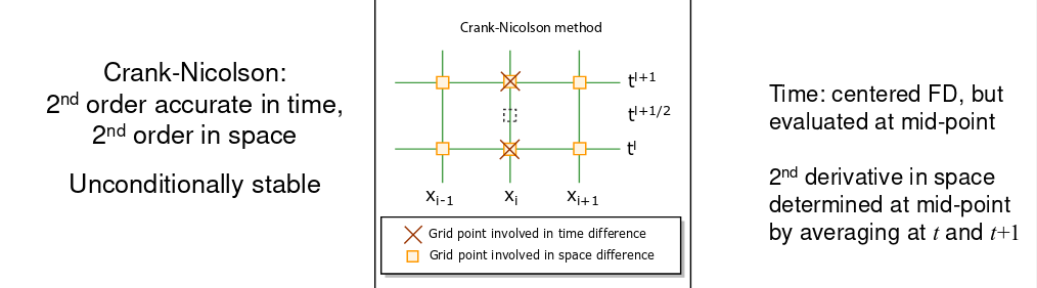
\includegraphics[scale=0.25]{cn}
	\end{center}
	\item This reduces the problem to a tridiagonal matrix solve which is trivial to solve. 
\end{itemize}
\end{frame}

\begin{frame}{Integration schemes in 2D}
\begin{itemize}
\item In 2D Fuhse et.al suggested the use of Alternating Direction Implicit\footnote{\cite{Fuhse_thesis}}. 
\item ADI is a 2 step process in which alternates between implicit and explicit derivates along the two dimensions. Each step now involves a tridiagonal matrix solution.
	\begin{center}
	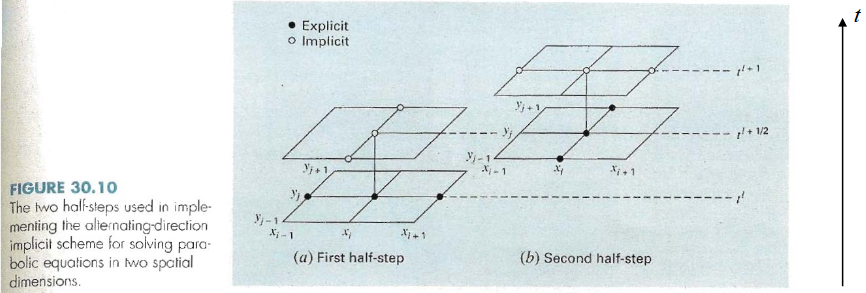
\includegraphics[scale=0.25]{adi}
	\end{center}
\end{itemize}
\end{frame}

\section{Review of previous work}
\begin{frame}{Previous work}
\begin{itemize}
	\item Fuhse et.al. chose IDL to implement the programs. 
	\item A more accurate version of the aforementioned scheme was implemented by Melchoir et.al.\footnote{\cite{Melchior17}} in C\texttt{++} with a Python front end. Although this was efficient, this implementation scheme involved writing the discretiztion routines for CN and ADI and thereby locked in the developers to these integration schemes.
	\item The schemes are straightforward to implement using the scipy.sparse libraries\footnote{https://github.com/s-sajid-ali/xwp}.
\end{itemize}
\end{frame}
	
\begin{frame}{FD vs Multislice}
\begin{itemize}
\item Multislice is better for free space propagation while FD gives better results for propagation through matter. \footnote{\cite{Melchior17}\cite{Scarmozzino91}}
\begin{center}
	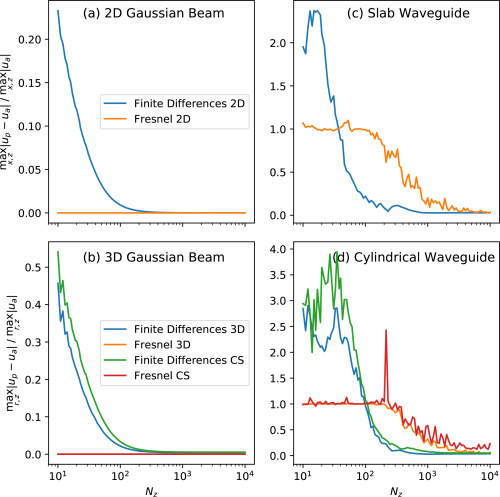
\includegraphics[scale=1.9]{fdms}
\end{center}
\end{itemize}
\end{frame}


\section{Current work}

\begin{frame}{PETSc overview}
\begin{itemize}
	\item What is PETSc ? 
	\\
		\qquad \textit{PETSc, pronounced PET-see (the S is silent), is a suite of data structures and routines for the scalable (parallel) solution of scientific applications modeled by partial differential equations}\footnote{https://www.mcs.anl.gov/petsc/}	\\
	\item Why use PETSc ?
	\\
		\qquad	PETSc can solve (in parallel) the linear system we have at hand using a large number of time-stepping integrations schemes, linear solver schemes and preconditioners which can be dynamically configured at runtime! Moreover, higher order finite volume schemes can be explored as well. An optimization library is also included\footnote{Finite difference is the defualt method to evaluate the jacobian, but since PETSc is written in C,  a source-to-source AD tool like Tapende can be used to give a function that evaluates the jacobian.}.
	\\
\end{itemize}
\end{frame}

\begin{frame}{PETSc architecture\footnote{https://www.mcs.anl.gov/petsc/documentation/tutorials/CSCS2010.pdf}}
\begin{center}
	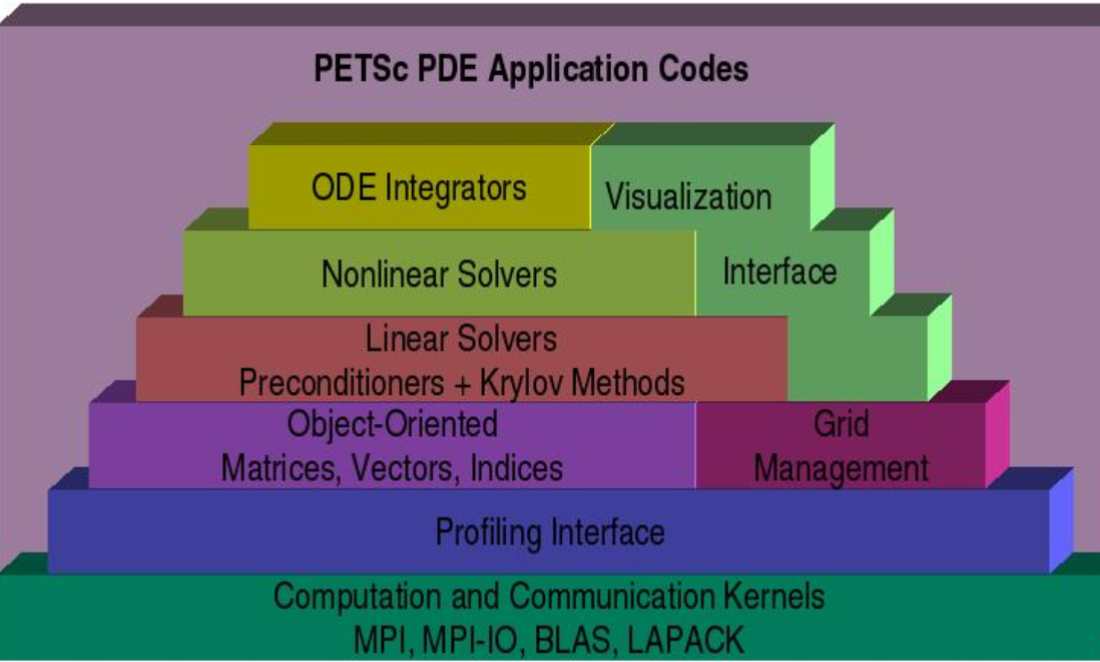
\includegraphics[scale=0.225]{petsc}
\end{center}
\end{frame}

\begin{frame}{Results 1D}
\begin{itemize}
\item Reproduce the plot of x-ray reflectivity from Kenan et.al\footnote{\cite{Li17}}, using FD/PETSc.
	\begin{center}
	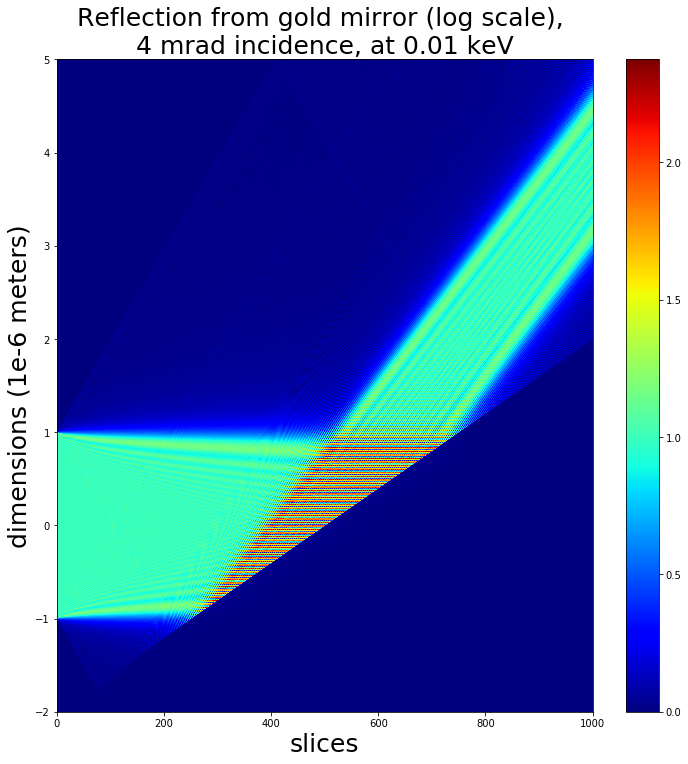
\includegraphics[scale=0.225]{petsc1d}
	\end{center}
\end{itemize}
\end{frame}




\begin{comment}
% Placing a * after \section means it will not show in the
% outline or table of contents.

\section*{Acknowledgements}

\begin{frame}{Acknowledgements}
  \begin{itemize}
  \item
    \alert{Chris Jacobsen} XSD, APS.
  \end{itemize}
\end{frame}

\end{comment}

% All of the following is optional and typically not needed. 
%\appendix
\renewcommand*{\bibfont}{\small}
\section{References}
\begin{frame}[t, allowframebreaks]
\frametitle{References}
\bibliographystyle{alpha}
\bibliography{fd}
\end{frame}

\end{document}

